
\chapter{Background }

This chapter will give the background needed to understand the core work of this thesis. 

\section{Foundations of Automatic and Interactive Theorem Proving} 
-

\section{Lean4 Foundations} 
\subsection{Bit Vector Support in Lean: BitVec and bv\_decide} 
\textbf{Bit Vectors in Lean:}
Bitvectors are fixed-width binary sequences that provide a mathematical abstraction for modeling machine-level data representation. A bitvector of width $w$ formally represents an element from the set $\{0, 1, \ldots, 2^w - 1\}$, which corresponds to the possible values that can be stored in a $w$-bit register. This representation is foundational in formal verification of hardware designs, instruction set architectures, and low-level software systems like compilers where bit vectors e.g enable reasoning about register operations. The Lean theorem prover supports reasoning about finite bit vectors through the \textit{BitVec} type, which represents a natural number \textit{n} with a proof that \( n < 2^w \). Specifcally \textit{BitVec} is implemented as "a wrapper around \textit{Fin} with a suitable bound". In Lean, the type \textit{Fin n} represents the finite set of natural numbers strictly less than n. An element of type \textit{Fin n} consist of a natural number \textit{val}, and a proof that \textit{val \( < \) n}. Both \textit{Fin} and  \textit{BitVec} exemplify Lean's dependent typing capabilities, as their type definitions depend on a value (the upper bound n or width w, respectively). \textit{Fin} itself is built upon \textit{Nat} (natural numbers), which have strong support in Lean's kernel.


\begin{lstlisting} [language=Lean, caption= bit vector represenation in Lean]
structure Fin (n : Nat) where
  val : Nat
  isLt : val < n 
-- type Fin n represents the finite set of natural numbers
strictly less than n, including a proof that val < n.

def BitVec (w : Nat) := { n : Nat // n < 2^w }
-- type BitVec represents the finite set of natural numbers
val, including a proof that n < 2^w.
\end{lstlisting}

 The design choice of wrapping the implementation of \textit{BitVec} around \textit{Fin} and \textit{Nat} allows for efficient reasoning about bit vectors by leveraging Lean's optimized natural number operations while maintaining the formal constraint of boundedness through dependent typing.
In compiled code, the representations of \textit{Fin, BitVec}  and \textit{Nat} are indistinguishable and efficient, leaving only the underlying natural number representation.

\noindent
\begin{lstlisting} [language=Lean, caption= Example of defining a Fin in the range of 0 to 31 with value 19 in Lean]
def exampleFin : Fin 32  :=  <19 , by simp [Nat.reduceLT]>
\end{lstlisting}
\begin{lstlisting} [language=Lean, caption= Example of defining a BitVec of width 32 with value 42 in Lean]
def bv32_ex1 : BitVec 32 :=  
            <42, by simp [Nat.reducePow, Nat.reduceLT]>
def bv32_ex2 : BitVec 32 :=  42#32
def bv32_ex3 : BitVec 32 :=  BitVec.ofNat 32 43 
\end{lstlisting}
 Lean provides multiple approaches for creating values of type \txtit{w} (Listing 2.3) . Whether a bit vector is interpreted as signed or unsigned depends on the bit vector operation used. Lean provides a comprehensive set of operations for both interpretations.

\textbf{Automated Reasoning with bv\_decide:}
To support automated reasoning about fixed-width bit vectors, Lean provides the \textit{bv\_decide} tactic. \textit{Bv\_decide}, a current research effort by the University of Cambridge, is a fully Lean 4-integrated tactic for solving fixed-width bit vector problems. The tactic targets proof goals involving fixed-width bit vector operations and booleans and automates proof goal resolution by combining various existing algorithms and techniques in theorem proving and automated reasoning (figure 2.1).

The bv\_decide tactic operates by processing the proof goal on multiple levels by combining internal processing with external  SMT solver integration. First, it applies standart Lean tactics to simplify and normalize the original proof goal. Then, it formulates a contradiction proof goal that is logically equivalent to the negation of the original goal. Next, the contradiction goal is bit blasted. Bitblasting is a process that decomposes bit vector operations into equivalent boolean operations. Then the bit-blasted goal is submitted to an external SMT solver. When the solver returns an UNSAT result, indicating the contradiction goal is unsatisfiable, the UNSAT certificate is reflected back into Lean's proof system. This certificate serves as evidence that the contradiction goal is false, which by logical equivalence confirms the truth of the original goal.

 The form of verification by reflecting external computation into a formal proof, is called \textit{proof by reflection}. In \textit{proof by reflection}, the result of a computation is integrated into a formal proof and seen as certificate for a proof. This in turn extends the trusted code base to the code generator that is invoked to compile and run the program that defines the computation.
\begin{figure}[htbp]
  \centering
  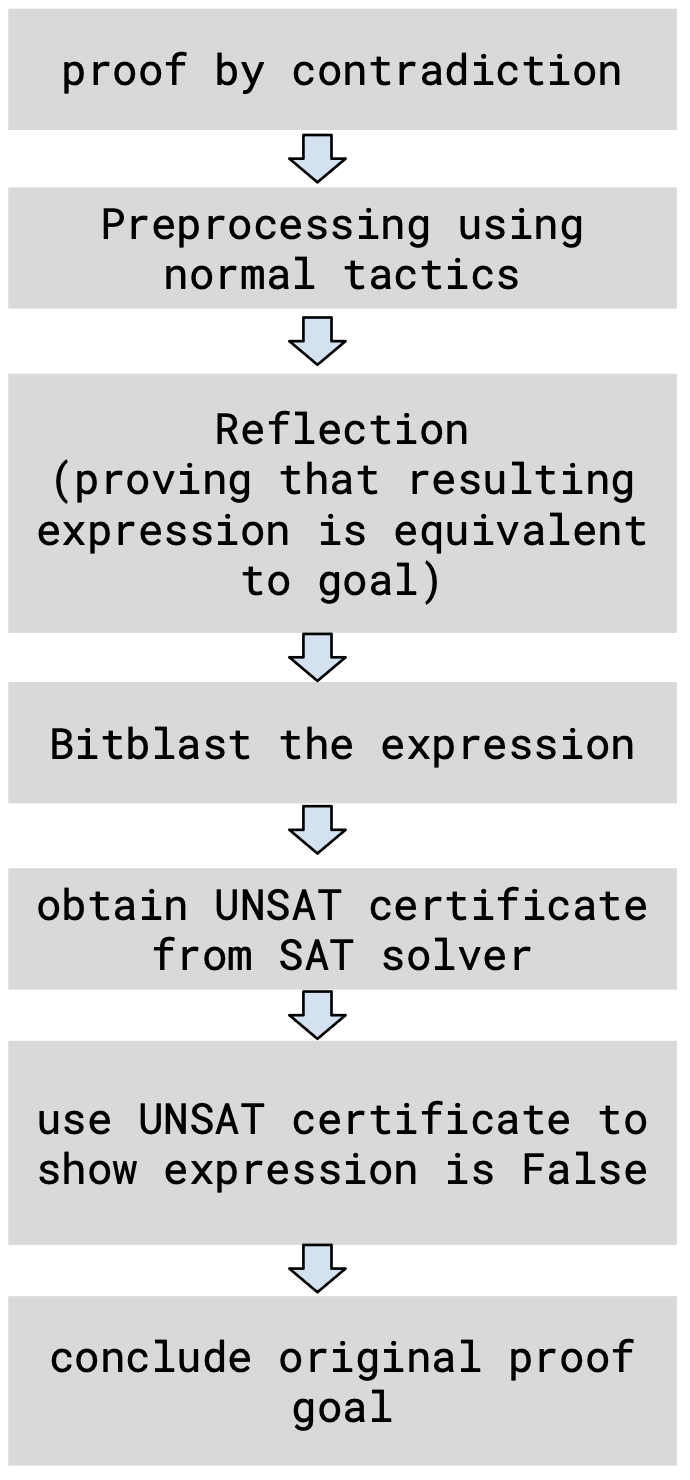
\includegraphics[scale=0.37]{thesis/bv_decide.png}
 
  \caption{Bv\_decide procedure flow}
  \label{fig:your-label}
\end{figure}

\textit{Contradiction Derivation}: Bv\_decide transforms the original goal into a contradiction form and starts a proof by contradiction. This allows for proving unsatisfiability of the contrary proof goal instead of forwards proving the original proof goal. 

\textit{Preprocessing}: Then bv\_decide normalizes and simplifies the goal by rewriting bit-vector expressions. It leverages rewrite rules inspired by the Bitwuzla SMT solver to perform these simplifications. Additionally, it performs and-flattening, which examines all currently available hypotheses, splits any conjunctions into individual hypotheses, and repeatedly applies rewriting across hypotheses until a fixed point is reached.

\textit{Reflection}: Proof by reflection is then used to show that transforming a bit-vector goal into a form where bit-vector operations are reified using additional Lean data structures preserves semantic equivalence. Wrapping bit-vector operations in these constructs enables easier processing in subsequent steps. The reflection proof guarantees that any proposition involving the enriched Lean representation is logically equivalent to a corresponding proposition about bit-vectors alone.

\textit{Bitblasting}: A verified bitblasting algorithm is then used to convert the reified bit-vector expression into an And-Inverter Graph (AIG), a data structure commonly used to efficiently represent Boolean circuits. This transformation reduces the high-level bit-vector goal to a low-level Boolean SAT problem. Finally, the AIG is translated into a conjunctive normal form (CNF) formula.

\textit{External Solving}: The CNF formula is sent to an external SMT solver, which attempts to produce an UNSAT certificate demonstrating that the formula is unsatisfiable. If the formula is satisfiable instead, the solver returns a counterexample.

\textit{Certificate Reflection}: If the SMT solver proves the formula is unsatisfiable (UNSAT), it returns an UNSAT certificate, which is imported back into Lean. The certificate is then checked within Lean ensuring that the unsatisfiability result is trustworthy and fully formalized.

\textit{Proof Construction}: Finally, the verified UNSAT certificate is used to construct a formal Lean proof of the original goal. Since the conjunction of the assumptions and the negation of the goal has been shown to be unsatisfiable, it logically follows that the original goal must be true. All previous proof steps are composed to conclude the overall proof.

Invoking the whole bv\_decide procedure to solve bit vector proof goals in Lean is illustrated below.
\begin{lstlisting} [language=python, caption= Discharging bit vector proof goal using bv\_decide]
theorem bv_add_comm {w : Nat} (a b : BitVec w) : BitVec.add a b 
    = BitVec.add b a := by
  bv_decide

theorem bv_mul_distr {w : Nat} (a b c : BitVec w) : 
  BitVec.mul a (BitVec.add b c) 
    = BitVec.add (BitVec.mul a b) (BitVec.mul a c) := by
  bv_decide
\end{lstlisting}

At the time of this thesis, bv\_decide handles a significant fragment of bit-vector logic and operations on bit vectors. However, it exhibits limitations in expressions that involve conversions between natural numbers and bit vectors, as natural numbers are unbounded in Lean and bit blasting requires a fixed-bounded width. Bv\_decide treats unknown variables or nonfixed-width bit vectors as undefined variables, however, yet attempts to resolve the goal within this abstraction. If the tactic fails to produce a proof, it returns a counterexample indicating which terms were treated as variables, providing insights into why the proof attempt failed(Listing 2.5). This interactive feedback exemplifies Lean's strength as an interactive theorem prover that leverages human-computer interaction to prove complex goals. This approach contrasts with common SMT solvers, which are proficient in solving fixed-width bit vector problems but do not support tools for interaction with the developer.


\begin{lstlisting} [language=python, caption= Example feedback by bv\_decide when trying to proof arbitrary-width bit vector theorem]
The prover found a potentially spurious counterexample:
- It abstracted the following unsupported expressions
as opaque variables: -- here the abstracted variables
will be listed.}
\end{lstlisting}





To enhance the performance of the bv\_decide procedure and avoid redundant calls to the external SMT solver, bv\_decide employs a caching mechanism for previously verified results. Additionally, the bv\_decide tactic has several configuration options to adapt its behavior to the specific structure of the proof goal e.g time-bound parameter that limits the solver execution. 

Invoking bv\_normalize instead of bv\_decide runs only the normalization step of bv\_decide  and is used in proof goals where automated algebraic normalization and simplification of bit vector terms without invoking the SAT solver suffices. If the proof goal is solved by bv\_normalize the SMT solver invocation and bit-blasting are skipped by bv\_decide. 
\section{Verified Instruction Selection and Peephole Optimizations } 
\subsection{Peephole Optimizations} 

\section{Llvm ir , Riscv and their semantics} 


\noindent
\begin{minipage}{0.6\textwidth}
\begin{lstlisting}[language=Python, caption=unoptimized]
int check(int x) {						        
	if (x == 0) return 0; 					
    else return x;
    def BitVec (w : Nat) := { n : Nat // n < 2^w }
}
\end{lstlisting}
\end{minipage}
\hfill
\begin{minipage}{0.45\textwidth}
\begin{lstlisting}[language=C, caption= optimzed assembly]
check: 
    mov r0, r0
}
\end{lstlisting}
\end{minipage}


\section {Semanctics}

